\lab{Data Structures II: Trees}{Data Structures II}
\label{lab:Python_DataStructures2}

\objective{Implement tree data structures and understand their relative strengths and weaknesses.}

\section*{Recursion}

Recursion is an important problem solving technique in computer programming.
A recursive function is one that calls itself.
When the function is executed, it continues calling itself until it reaches a specified base case.
Then the function exits without calling itself again, and each previous function call is resolved.
As a simple example, suppose we want to recursively sum all positive integers from $1$ to some integer $n$.

\begin{lstlisting}
def recursive_sum(n):
	"""Calculate the sum of all positive integers in [1, n] recursively."""

	# Typically the base case comes first. There are no positive integers less
	# than 1, so if 'n' is 1 we stop the recursion and return 1 (since the sum of
	# all integers in [1, 1] is 1).
	if n == 1:
		return 1

	# If the base case hasn't been reached, the function recurses by calling
	# itself on the next smallest integer and adding 'n'.
	else:
		return n + recursive_sum(n-1)
\end{lstlisting}

The computer calculates \li{recursive_sum(5)} with a sequence of function calls.

\begin{lstlisting}
# To find the recursive_sum(5), we need to calculate recursive_sum(4).
# But to find recursive_sum(4), we need to calculate recursive_sum(3).
# This continues until the base case is reached.

recursive_sum(5)		# return 5 + recursive_sum(4)
	recursive_sum(4)		# return 4 + recursive_sum(3)
		recursive_sum(3)		# return 3 + recursive_sum(2)
			recursive_sum(2)		# return 2 + recursive_sum(1)
				recursive_sum(1)		# Base case: return 1.
\end{lstlisting}

Now that we've reached a base case, we can unwind the recursion.
Reading from bottom to top, we substitute the values that result from each function call.

\begin{lstlisting}
recursive_sum(5)		# 5 + 10 = 15
	recursive_sum(4)		# 4 + 6 = 10
		recursive_sum(3)		# 3 + 3 = 6
			recursive_sum(2)		# 2 + 1 = 3
				recursive_sum(1)		# Base case: return 1.
\end{lstlisting}

So \li{recursive_sum(5)} returns 15 (which is correct, since $1 + 2 + 3 + 4 + 5 = 15$).
Many problems that can be solved by iterative methods can also be solved (often more efficiently) with a recursive approach.
Compare, for example, the following two methods for calculating the $n^{th}$ Fibonacci number.

\begin{lstlisting}
def iterative_fib(n):
	"""Calculate the nth Fibonacci number iteratively."""
	fibonacci = list()		# Initialize an empty list.
	fibonacci.append(0)		# append 0 (the 0th Fibonacci number).
	fibonacci.append(1)		# append 1 (the 1st Fibonacci number).
	for i in range(1, n):
		# Starting at the third entry, calculate the next number
		# by adding the last two entries in the list.
		fibonacci.append(fibonacci[-1] + fibonacci[-2])
	# When the entire list has been loaded, return the nth entry.
	return fibonacci[n]

def recursive_fib(n):
	"""Calculate the nth Fibonacci number recursively."""
	# The base cases are the first two Fibonacci numbers.
	if n == 0:				# Base case 1: the 0th Fibonacci number is 0.
		return 0
	elif n == 1:			# Base case 2: the 1st Fibonacci number is 1.
		return 1
	# If we haven't reached a base case, the function recurses by calling
	# itself on the previous two Fibonacci numbers.
	else:
		return recursive_fib(n-1) + recursive_fib(n-2)
\end{lstlisting}

This time, the sequence of function calls is slightly more complicated because \li{recursive_fib} calls itself twice until a base case is reached.

\begin{lstlisting}
recursive_fib(5)		# The original call makes two additional calls:
	recursive_fib(4)		# this one...
		recursive_fib(3)
			recursive_fib(2)
				recursive_fib(1)		# Base case 2: return 1
				recursive_fib(0)		# Base case 1: return 0
			recursive_fib(1)		# Base case 2: return 1
		recursive_fib(2)
			recursive_fib(1)		# Base case 2: return 1
			recursive_fib(0)		# Base case 1: return 0
	recursive_fib(3)		# ...and this one.
		recursive_fib(2)
			recursive_fib(1)		# Base case 2: return 1
			recursive_fib(0)		# Base case 1: return 0
		recursive_fib(1)		# Base case 2: return 1
\end{lstlisting}

The sum of all of the base case results, from top to bottom, is $1 + 0 + 1 + 1 + 0 + 1 + 0 + 1 = 5$, so \li{recursive_fib(5)} returns 5 (correctly).
The key to recursion is understanding the base cases correctly and making correct recursive calls.

% Problem 1: simple recursion for linked lists traversal
\begin{problem}
Rewrite the following iterative function for finding data in a linked list using recursion.
Use the basic linked list object from the previous lab to test the function (copy \li{LinkedLists.py} into your folder and import the \li{LinkedList} class).
\begin{lstlisting}
# solutions.py

def iterative_search(linkedlist, data):
	current = linkedlist.head
	while current is not None:
		if current.data == data:
			return current
		current = current.next
	raise ValueError(str(data) + " is not in the list.")
\end{lstlisting}
(Hint: define an inner function to perform the actual recursion)
\end{problem}

\begin{warn}
It is not always better to rewrite an iterative method recursively.
In Python, a function may only call itself 999 times.
On the $1000^{th}$ call, a \li{RuntimeError} is raised to prevent a stack overflow.
Whether or not recursion is appropriate depends on the problem to be solved and the algorithm to solve it.
\end{warn}

\section*{Trees}

A \emph{tree} data structure is a specialized linked list.
Trees are more difficult to build than standard linked lists, but they are almost always more efficient.
While the computational complexity of finding a node in a linked list is $O(n)$, a well-built, balanced tree will find a node with a complexity of $O(\log{n})$.
Some types of trees can be constructed quickly but take longer to retrieve data, while others take more time to build and less time to retrieve data.

The first node in a tree is called the \emph{root}.
The root node points to other nodes, called children.
Each child node in turn points to its children.
This continues on each branch until its end is reached.
A node with no children is called a \emph{leaf node}.

Mathematically, a tree is a directed graph with no cycles.
Therefore a linked lists qualifies as a tree, albeit a boring one.
The head node is the root node, and it has one child node.
That child node also has one child node, which in turn has one child.
This continues until the end of the list, with the last node as the only leaf node.

Other kinds of trees may be more complicated.
See Figure \ref{fig:trees}.

\begin{figure}
\begin{tikzpicture}[
    level 1/.style={sibling distance=2cm},
    level 2/.style={sibling distance=20mm}]

    \node [circle,draw] (4){4}
        child {node[draw, circle] (5) {5} edge from parent[draw=none]}
        child {node[circle,draw] (3) {3}edge from parent[draw=none]
        child{node[draw,circle](2){2}edge from parent[draw=none]}
        child{node[circle, draw](7){7}edge from parent[draw=none]}
        };
    \node [draw=none, node distance=.1cm] (4a)[above of=4]{}
        child {node[draw=none] (5a) {} edge from parent[draw=none]}
        child {node[draw=none] (3a) {}edge from parent[draw=none]
        child{node[draw=none](2a){}edge from parent[draw=none]}
        child{node[draw=none](7a){}edge from parent[draw=none]}
        };
    \node [draw=none, node distance=.1cm] (4b)[below of=4]{}
        child {node[draw=none] (5b) {} edge from parent[draw=none]}
        child {node[draw=none] (3b) {}edge from parent[draw=none]
        child{node[draw=none](2b){}edge from parent[draw=none]}
        child{node[draw=none](7b){}edge from parent[draw=none]}
        };
\foreach \s/\t in {4a/5a, 4a/3a, 5a/2a, 3a/7a} 
    {\draw[->, >=stealth', shorten <=.23cm, shorten >=.1cm](\s)--(\t);}

\end{tikzpicture}
\qquad
\begin{tikzpicture}[
    auto,
    level 1/.style={sibling distance=2cm},
    level 2/.style={sibling distance=20mm}]

    \node [circle,draw] (5a){5}
        child {node[circle,draw] (2a) {2}edge from parent[draw=none]
            child { node[circle,draw] (1a) {1}edge from parent[draw=none]}
            child {node[draw = none] (invisble){} edge from parent[draw=none]}     
        }
        child {node[circle,draw] (7a) {7}edge from parent[draw=none]
        child{node[circle, draw](6a){6}edge from parent[draw=none]}
        child{node[circle, draw](8a){8}edge from parent[draw=none]}
        };
    \node [draw=none, node distance=.1cm] (i5a)[above of=5a]{}
        child {node[draw=none] (i2a) {}edge from parent[draw=none]
            child { node[draw=none] (i1a) {}edge from parent[draw=none]}
            child {node[draw = none] (invisbleA){} edge from parent[draw=none]}     
        }
        child {node[draw=none] (i7a) {}edge from parent[draw=none]
        child{node[draw=none](i6a){}edge from parent[draw=none]}
        child{node[draw=none](i8a){}edge from parent[draw=none]}
        };
\foreach \s/\t in {i5a/i2a, i5a/i7a} 
    {\draw[->, >=stealth', shorten <=.23cm, shorten >=.1cm](\s)--(\t);}
\foreach \s/\t in {i2a/i1a, i7a/i6a, i7a/i8a}
    {\draw[->, >=stealth', shorten <=.27cm, shorten >=.1cm](\s)--(\t);}
\end{tikzpicture}
\caption{Both of these graphs are trees, but only the tree on the right is a binary search tree. How could the graph on the left be altered to make it a BST?}
\label{fig:trees}
\end{figure}

\section*{Binary Search Trees}

A \emph{binary search tree} (BST) data structure is a tree that allows each node to have up to two children, usually called \li{left} and \li{right}.
The left child of a node contains data that is less than its parent node's data.
The right child's data is greater.

The tree on the right in Figure \ref{fig:trees} is an example of a of binary search tree.
In practice, binary search tree nodes have attributes that keep track of their data, their children, and (in doubly-linked trees) their parent.

\begin{lstlisting}
# Trees.py

class BSTNode(object):
    """A Node class for Binary Search Trees. Contains some data, a
    reference to the parent node, and references to two child nodes.
    """
    def __init__(self, data):
        """Construct a new node and set the data attribute. The other
        attributes will be set when the node is added to a tree.
        """
        self.data = data
        self.prev = None        # A reference to this node's parent node.
        self.left = None        # This node's data will be less than self.data
        self.right = None       # This node's data will be greater than self.data
        
    def __str__(self):
        """String representation: the data contained in the node."""
        return str(self.data)
\end{lstlisting}

The actual binary search tree class has an attribute pointing to its root.

\begin{lstlisting}
# Trees.py

class BST(object):
    """Binary Search Tree data structure class.
    The first node is referenced to by 'root'.
    """
    def __init__(self):
        """Initialize the root attribute."""
        self.root = None
\end{lstlisting}

\subsection*{Finding in a Binary Search Tree}

Many tree algorithms are best understood and implemented using recursion.
For instance, finding a node in a binary search tree can be done recursively.
Starting at the root, we check if the data we are looking for matches the current node.
If it does not, then if the data is less than the current node's data we search again on the left child.
If the data is greater, we search on the right child.
This process continues until the data is found or, if the data is not in the tree, an empty child is searched.
Carefully read the following code; similar techniques will be used for subsequent methods.

\begin{lstlisting}
class BST(object):
    # ...

    def find(self, data):
        """Return the node containing 'data'. If there is no such node in the
        tree, raise a ValueError with error message "<data> is not in the tree."
        """
        # First, check to see if the tree is empty.
        if self.root is None:
            raise ValueError(str(data) + " is not in the tree.")
        
        # Define a recursive function to traverse the tree.
        def _step(current, item):
            """Recursively step through the tree until the node containing
            'item' is found. If there is no such node, raise a Value Error.
            """
            if current is None:                 # Base case 1: dead end.
                raise ValueError(str(data) + " is not in the tree.")
            if item == current.data:            # Base case 2: the data matches.
                return current
            if item < current.data:             # Step to the left
                return _step(current.left,item)
            else:                               # Step to the right
                return _step(current.right,item)
        
        # Start the recursion on the root of the tree.
        return _step(self.root, data)
\end{lstlisting}

\begin{info}
Conceptually, each node of a BST partitions the data of its subtree into two halves: the data that is less than the parent, and the data that is greater.
We can extend this concept to multiple dimensions (see the K-D Trees lab).
\end{info}

\subsection*{Inserting to a Binary Search Tree}

To insert new data into a binary search tree, a leaf node is added at the correct location.
First, we find the node that should be the parent of the new node.
We find the parent recursively, using a similar approach to the \li{find} method.
Once the correct parent is found, the new node is added as the left or right child of the parent.
See Figure \ref{fig:BST.insertion} for an example.

\begin{figure}
\begin{tikzpicture}[
    auto,
    level 1/.style={sibling distance=2cm},
    level 2/.style={sibling distance=20mm}]

    \node [circle,draw] (5a){5}
        child {node[circle,draw] (2a) {2}edge from parent[draw=none]
            child { node[circle,draw] (1a) {1}edge from parent[draw=none]}
            child {node[draw = none] (invisble){} edge from parent[draw=none]}     
        }
        child {node[circle,draw] (7a) {7}edge from parent[draw=none]
        child{node[circle, draw](3a){3}edge from parent[draw=none]}
        child{node[circle, draw](8a){8}edge from parent[draw=none]}
        };
    \node [draw=none, node distance=.1cm] (i5a)[above of=5a]{}
        child {node[draw=none] (i2a) {}edge from parent[draw=none]
            child { node[draw=none] (i1a) {}edge from parent[draw=none]}
            child {node[draw = none] (invisbleA){} edge from parent[draw=none]}     
        }
        child {node[draw=none] (i7a) {}edge from parent[draw=none]
        child{node[draw=none](i3a){}edge from parent[draw=none]}
        child{node[draw=none](i8a){}edge from parent[draw=none]}
        };
    \node [draw=none, node distance=.1cm] (i5b)[below of=5a]{}
        child {node[draw=none] (i2b) {}edge from parent[draw=none]
            child { node[draw=none] (i1b) {}edge from parent[draw=none]}
            child {node[draw = none] (invisbleB){} edge from parent[draw=none]}     
        }
        child {node[draw=none] (i7b) {}edge from parent[draw=none]
        child{node[draw=none](i3b){}edge from parent[draw=none]}
        child{node[draw=none](i8b){}edge from parent[draw=none]}
        };
\node [draw=none, node distance=1.5cm](root)[above right of=5a]{root};
\draw[->, >=stealth', shorten >= .1cm](root)--(5a);
\node [draw=none, node distance=1.5cm](current)[above left of=5a]{current};
\draw[->, >=stealth', shorten >= .1cm](current)--(5a);
\foreach \s/\t in {i5a/i2a, i2b/i5b, i5a/i7a, i7b/i5b} 
    {\draw[->, >=stealth', shorten <=.23cm, shorten >=.1cm](\s)--(\t);}
\foreach \s/\t in {i2a/i1a, i1b/i2b, i7a/i8a, i8b/i7b}
    {\draw[->, >=stealth', shorten <=.27cm, shorten >=.1cm](\s)--(\t);}
\end{tikzpicture}
\qquad
\begin{tikzpicture}[
    auto,
    level 1/.style={sibling distance=2cm},
    level 2/.style={sibling distance=20mm}]

    \node [circle,draw] (5a){5}
        child {node[circle,draw] (2a) {2}edge from parent[draw=none]
            child { node[circle,draw] (1a) {1}edge from parent[draw=none]}
            child {node[draw = none] (invisble){} edge from parent[draw=none]}     
        }
        child {node[circle,draw] (7a) {7}edge from parent[draw=none]
        child{node[circle, draw](3a){3}edge from parent[draw=none]}
        child{node[circle, draw](8a){8}edge from parent[draw=none]}
        };
    \node [draw=none, node distance=.1cm] (i5a)[above of=5a]{}
        child {node[draw=none] (i2a) {}edge from parent[draw=none]
            child { node[draw=none] (i1a) {}edge from parent[draw=none]}
            child {node[draw = none] (invisbleA){} edge from parent[draw=none]}     
        }
        child {node[draw=none] (i7a) {}edge from parent[draw=none]
        child{node[draw=none](i3a){}edge from parent[draw=none]}
        child{node[draw=none](i8a){}edge from parent[draw=none]}
        };
    \node [draw=none, node distance=.1cm] (i5b)[below of=5a]{}
        child {node[draw=none] (i2b) {}edge from parent[draw=none]
            child { node[draw=none] (i1b) {}edge from parent[draw=none]}
            child {node[draw = none] (invisbleB){} edge from parent[draw=none]}     
        }
        child {node[draw=none] (i7b) {}edge from parent[draw=none]
        child{node[draw=none](i3b){}edge from parent[draw=none]}
        child{node[draw=none](i8b){}edge from parent[draw=none]}
        };
\node [draw=none, node distance=1.5cm](root)[above right of=5a]{root};
\draw[->, >=stealth', shorten >= .1cm](root)--(5a);
\node [draw=none, node distance=1.5cm](current)[above left of=2a]{current};
\draw[->, >=stealth', shorten >= .1cm](current)--(2a);
\foreach \s/\t in {i5a/i2a, i2b/i5b, i5a/i7a, i7b/i5b} 
    {\draw[->, >=stealth', shorten <=.23cm, shorten >=.1cm](\s)--(\t);}
\foreach \s/\t in {i2a/i1a, i1b/i2b, i2a/i3a, i3b/i2b, i7a/i8a, i8b/i7b}
    {\draw[->, >=stealth', shorten <=.27cm, shorten >=.1cm](\s)--(\t);}
\end{tikzpicture}
\caption{To insert a node containing 3 to the BST on the left, start `current' at the root and recurse down the tree until it points to the node that should be 3's parent. Connect that parent to the child, then the child to its new parent.}
\label{fig:BST.insertion}
\end{figure}

% Some pseudocode to help with insertion, if deemed necessary.
\begin{comment}
\begin{lstlisting}
"""Pseudocode for finding the correct parent of a new node

find the parent of node, data
	if data < node.data:
		if node.left is not None 
			find the parent of node.left, data
		else:
			return node
	if data > node.right:
		if data > node.data:
			if node.right is not None:
				find the parent of node.right, data
			else:
				return node
"""
\end{lstlisting}
\end{comment}

% Problem 2: BST.insert()
\begin{problem}
Implement the \li{insert} method in the \li{BST} class.
To accomplish this, write a recursive \li{_find_parent} method within \li{insert}.
Find the correct parent, then determine whether the new node will be its left or right child.
Then double-link the parent and the new child.
Be sure to consider the special case of inserting to an empty tree.
To test your tree, use (but do not modify) the provided \li{BST.__str__} method.

Do not allow for duplicates in the tree: if the user executes \li{insert(x)} and there is already a node in the tree containing \li{x}, raise a ValueError.
\end{problem}

\subsection*{Removing from a Binary Search Tree}

Deleting nodes from a binary search tree is more difficult than searching and inserting.
Insertion always creates a new leaf node, but removal may delete any kind of node.
This leads to several different cases to consider.

\subsubsection*{Removing a leaf node}

In Python, an object is automatically deleted if there are no references to it.
Call the node to be removed the \emph{target node}, and suppose it has no children.
To remove the target, find the target's parent, then delete the parent's reference to the target.
Then there are no references to the target, so the target node is deleted.
Since the target is a leaf node, removing it does not affect the rest of the tree structure.

\begin{comment}
\begin{lstlisting}
"""Pseudocode for removing a leaf node
if the target node does not have children:
	if the target's data is smaller than its parent's data:
		set the parent's left child to None
	else:
		set the parent's right child to None
"""
\end{lstlisting}
\end{comment}

\subsubsection*{Removing a node with one child}

If the target node has one or more children, we must be careful not to delete the children when the target is removed.
Simply removing the target as if it were a leaf node would delete the entire subtree originating from the target.

To avoid deleting all of the target's descendents, we point the target's parent to an appropriate successor.
If the target has only one child, then that child is the successor.
Connect the target's parent to the successor, and double-link by setting the successor's parent to be the target node's parent.
Then, since the target has no references pointing to it, it is deleted.
The target's successor, however, is pointed to by the target's parent, and so it remains in the tree.

\begin{figure}
\begin{tikzpicture}[
    auto,
    level 1/.style={sibling distance=2cm},
    level 2/.style={sibling distance=20mm}]

    \node [circle,draw] (5){5}
        child {node[circle,draw] (2) {2}edge from parent[draw=none]
            child { node[circle,draw] (1) {1}edge from parent[draw=none]
            child{node[draw=none](invisible){} edge from parent[draw=none]}
            child{node[draw,circle](3){3} edge from parent[draw=none]}
       }
            child {node[draw, circle] (4){4} edge from parent[draw=none]}     
        }
    child {node[circle,draw] (9a) {9}edge from parent[draw=none]
        child{node[draw=none](8){}edge from parent[draw=none]}
        };
    \node [draw=none, node distance=.1cm] (5a)[above of=5]{}
        child {node[draw=none] (2a) {}edge from parent[draw=none]
            child { node[draw=none] (1a) {}edge from parent[draw=none]
            child{node[draw=none](invisibleA){} edge from parent[draw=none]}
            child{node[draw=none](3a){} edge from parent[draw=none]}
        }
            child {node[draw = none] (4a){} edge from parent[draw=none]}     
        }
        child {node[draw=none] (9a) {}edge from parent[draw=none]
        child{node[draw=none](8a){}edge from parent[draw=none]}
        };

    \node [draw=none, node distance=.1cm] (5b)[below of=5]{}
        child {node[draw=none] (2b) {}edge from parent[draw=none]
            child { node[draw=none] (1b) {}edge from parent[draw=none]
            child{node[draw=none](invisibleB){} edge from parent[draw=none]}
            child{node[draw=none](3b){} edge from parent[draw=none]}
        }
            child {node[draw = none] (4b){} edge from parent[draw=none]}     
        }
        child {node[draw=none] (9b) {}edge from parent[draw=none]
        child{node[draw=none](8b){}edge from parent[draw=none]}
        };
\node [draw=none, node distance=2cm](current)[left of=5a]{current};
\draw[->, >=stealth', shorten >= .2cm](current)--(5a);
\foreach \s/\t in {2a/1a, 1b/2b, 2a/4a, 4b/2b, 5a/2a, 2b/5b, 5a/9a, 9b/5b, 4a/3a, 3b/4b} 
    {\draw[->, >=stealth', shorten <=.23cm, shorten >=.1cm](\s)--(\t);}
\end{tikzpicture}
\qquad
\begin{tikzpicture}[
    auto,
    level 1/.style={sibling distance=2cm},
    level 2/.style={sibling distance=20mm}]

    \node [circle,draw] (5){5}
        child {node[circle,draw] (2) {2}edge from parent[draw=none]
            child { node[circle,draw] (1) {1}edge from parent[draw=none]
            child{node[draw=none](invisible){} edge from parent[draw=none]}
            child{node[draw,circle](3){3} edge from parent[draw=none]}
       }
            child {node[draw, circle] (4){4} edge from parent[draw=none]}     
        }
    child {node[circle,draw] (9a) {9}edge from parent[draw=none]
        child{node[draw=none](8){}edge from parent[draw=none]}
        };
    \node [draw=none, node distance=.1cm] (5a)[above of=5]{}
        child {node[draw=none] (2a) {}edge from parent[draw=none]
            child { node[draw=none] (1a) {}edge from parent[draw=none]
            child{node[draw=none](invisibleA){} edge from parent[draw=none]}
            child{node[draw=none](3a){} edge from parent[draw=none]}
        }
            child {node[draw = none] (4a){} edge from parent[draw=none]}     
        }
        child {node[draw=none] (9a) {}edge from parent[draw=none]
        child{node[draw=none](8a){}edge from parent[draw=none]}
        };

    \node [draw=none, node distance=.1cm] (5b)[below of=5]{}
        child {node[draw=none] (2b) {}edge from parent[draw=none]
            child { node[draw=none] (1b) {}edge from parent[draw=none]
            child{node[draw=none](invisibleB){} edge from parent[draw=none]}
            child{node[draw=none](3b){} edge from parent[draw=none]}
        }
            child {node[draw = none] (4b){} edge from parent[draw=none]}     
        }
        child {node[draw=none] (9b) {}edge from parent[draw=none]
        child{node[draw=none](8b){}edge from parent[draw=none]}
        };
\node [draw=none, node distance=2cm](current)[left of=2a]{current};
\draw[->, >=stealth', shorten >= .2cm](current)--(2a);
\node [draw=none, node distance=2cm](successor)[right of=3a]{successor};
\draw[->, >=stealth', shorten >= .2cm](successor)--(3a);
\foreach \s/\t in {2a/1a, 1b/2b, 2a/4a, 4b/2b, 5a/2a, 2b/5b, 5a/9a, 9b/5b, 4a/3a, 3b/4b} 
    {\draw[->, >=stealth', shorten <=.23cm, shorten >=.1cm](\s)--(\t);}
\end{tikzpicture}
\qquad
\begin{tikzpicture}[
    auto,
    level 1/.style={sibling distance=2cm},
    level 2/.style={sibling distance=20mm}]

    \node [circle,draw] (5){5}
        child {node[circle,draw] (2) {2}edge from parent[draw=none]
            child { node[circle,draw] (1) {1}edge from parent[draw=none]
            child{node[draw=none](invisible){} edge from parent[draw=none]}
            child{node[draw,circle](3){3} edge from parent[draw=none]}
       }
            child {node[draw, circle] (4){4} edge from parent[draw=none]}     
        }
    child {node[circle,draw] (9a) {9}edge from parent[draw=none]
        child{node[draw=none](8){}edge from parent[draw=none]}
        };
    \node [draw=none, node distance=.1cm] (5a)[above of=5]{}
        child {node[draw=none] (2a) {}edge from parent[draw=none]
            child { node[draw=none] (1a) {}edge from parent[draw=none]
            child{node[draw=none](invisibleA){} edge from parent[draw=none]}
            child{node[draw=none](3a){} edge from parent[draw=none]}
        }
            child {node[draw = none] (4a){} edge from parent[draw=none]}     
        }
        child {node[draw=none] (9a) {}edge from parent[draw=none]
        child{node[draw=none](8a){}edge from parent[draw=none]}
        };

    \node [draw=none, node distance=.1cm] (5b)[below of=5]{}
        child {node[draw=none] (2b) {}edge from parent[draw=none]
            child { node[draw=none] (1b) {}edge from parent[draw=none]
            child{node[draw=none](invisibleB){} edge from parent[draw=none]}
            child{node[draw=none](3b){} edge from parent[draw=none]}
        }
            child {node[draw = none] (4b){} edge from parent[draw=none]}     
        }
        child {node[draw=none] (9b) {}edge from parent[draw=none]
        child{node[draw=none](8b){}edge from parent[draw=none]}
        };
\node [draw=none, node distance= 2cm](current)[left of=2a]{current};
\draw[->, >=stealth', shorten >= .2cm](current)--(2a);
\node [draw=none, node distance=2cm](successor)[right of=3a]{successor};
\draw[->, >=stealth', shorten >= .2cm](successor)--(3a);
\foreach \s/\t in {2a/1a, 1b/2b, 2a/4a, 4b/2b, 5a/2a, 2b/5b, 5a/9a, 9b/5b} 
    {\draw[->, >=stealth', shorten <=.23cm, shorten >=.1cm](\s)--(\t);}
\end{tikzpicture}
\qquad
\begin{tikzpicture}[
    auto,
    level 1/.style={sibling distance=2cm},
    level 2/.style={sibling distance=20mm}]

    \node [circle,draw] (5){5}
        child {node[circle,draw] (2) {3}edge from parent[draw=none]
            child { node[circle,draw] (1) {1}edge from parent[draw=none]
            child{node[draw=none](invisible){} edge from parent[draw=none]}
            child{node[draw,circle](3){2} edge from parent[draw=none]}
       }
            child {node[draw, circle] (4){4} edge from parent[draw=none]}     
        }
    child {node[circle,draw] (9a) {9}edge from parent[draw=none]
        child{node[draw=none](8){}edge from parent[draw=none]}
        };
    \node [draw=none, node distance=.1cm] (5a)[above of=5]{}
        child {node[draw=none] (2a) {}edge from parent[draw=none]
            child { node[draw=none] (1a) {}edge from parent[draw=none]
            child{node[draw=none](invisibleA){} edge from parent[draw=none]}
            child{node[draw=none](3a){} edge from parent[draw=none]}
        }
            child {node[draw = none] (4a){} edge from parent[draw=none]}     
        }
        child {node[draw=none] (9a) {}edge from parent[draw=none]
        child{node[draw=none](8a){}edge from parent[draw=none]}
        };

    \node [draw=none, node distance=.1cm] (5b)[below of=5]{}
        child {node[draw=none] (2b) {}edge from parent[draw=none]
            child { node[draw=none] (1b) {}edge from parent[draw=none]
            child{node[draw=none](invisibleB){} edge from parent[draw=none]}
            child{node[draw=none](3b){} edge from parent[draw=none]}
        }
            child {node[draw = none] (4b){} edge from parent[draw=none]}     
        }
        child {node[draw=none] (9b) {}edge from parent[draw=none]
        child{node[draw=none](8b){}edge from parent[draw=none]}
        };
\node [draw=none, node distance=2cm](current)[left of=2a]{current};
\draw[->, >=stealth', shorten >= .2cm](current)--(2a);
\node [draw=none, node distance=2cm](successor)[right of=3a]{successor};
\draw[->, >=stealth', shorten >= .2cm](successor)--(3a);
\foreach \s/\t in {2a/1a, 1b/2b, 2a/4a, 4b/2b, 5a/2a, 2b/5b, 5a/9a, 9b/5b} 
    {\draw[->, >=stealth', shorten <=.23cm, shorten >=.1cm](\s)--(\t);}
\end{tikzpicture}
\caption{To remove the node containing 2 from the top left BST, start `current' at the root (upper left) and recurse down the tree until it points to the target. Then locate the in-order successor (upper right) and delete it (lower left, recording its data. Finally, swap the data in the target with the data that was in the successor (lower right).}
\label{fig:BST.remove_twoChild}
\end{figure}

\begin{comment}
\begin{lstlisting}
"""Pseudocode for removing a node with one child
if the target node has one child:
	if target.parent.right is the target:
		set parent's right child to the target's child.
	if target.parent.left is the target:
		set parent's left child to the target's child.
"""
\end{lstlisting}
\end{comment}

\subsubsection*{Removing a node with two children}

Removal is more complicated if the target node has two children.
To delete this kind of node, first we find it's immediate in-order successor.
This successor is the node with the smallest data that is larger than the target's data.
It may be found by moving to the right child of the target (so that it's value is greater than the target's value), and then to the left for as long as possible (so that it has the smallest such value).
Note that because of how the successor is chosen, any in-order successor can only have at most one child.

Once the successor is found, the target and its successor must switch places in the graph, and then the target must be removed.
This can be done by simply switching the data values for the target and its successor.
Then the node with the target data has at most one child, and may be deleted accordingly.
If the successor was chosen appropriately, then the binary search tree structure and ordering will be maintained once the deletion is finished.

The easiest way to implement this is to use recursion.
First, because the successor has at most one child, we may recursivley remove the successor node by calling \li{remove} on the successor's data.
Then set the data stored in the target node as the successor's data.
See Figure \ref{fig:BST.remove_twoChild}.

\begin{comment}
\begin{lstlisting}
"""Pseudocode for removing a node with two children.

find the successor:
	set the current node to be target.left
	set current to be current.right until there is no right child
	return current.

Remove the node that has the successor's data (it will only have one child).
Change the target's data to the successor's data.
"""
\end{lstlisting}
\end{comment}

\subsubsection*{Removing the root node}

In each of the above cases, we must also consider the subcase where the target is the root node.
If the root has no children, resetting the root or calling the constructor will do.
If the root has one child, that child becomes the new root of the tree.
If the root has two children, the successor becomes the new root of the tree.

% Problem 3: BST.remove()
\begin{problem}
Implement the \li{remove} method in the \li{BST} class.
If the tree is empty, or if the target node is not in the tree, raise a \li{ValueError}.

Make sure to cover all possible cases:
\begin{enumerate}
\item The tree is empty (\li{ValueError})
\item The target is not in the tree (\li{ValueError})
\item The target is the root node:
	\begin{enumerate}
	\item{the root is a leaf node, hence the only node in the tree}
	\item{the root has one child}
	\item{the root has two children}
	\end{enumerate}
\item The target is in the tree but is not the root:
	\begin{enumerate}
	\item{the target is a leaf node}
	\item{the target has one child}
	\item{the target has two children}
	\end{enumerate}
\end{enumerate}
Test your solution thoroughly with each case.

(Hint: use \li{find} wherever appropriate.)
\end{problem}

There are many variations on the binary search tree, each with their own particular advantages and disadvantages.
The reader is encouraged to research \href{https://en.wikipedia.org/wiki/B-tree}{B-trees}, \href{https://en.wikipedia.org/wiki/Red%E2%80%93black_tree}{red-black trees}, and \href{https://en.wikipedia.org/wiki/Splay_tree}{splay trees}.
We conclude with a discussion of one of the most famous BST variants: the AVL.

\section*{AVL Trees}

Binary search trees are a good way of organizing data so that it is quickly accessible.
However, pathologies may arise when certain data sets are stored using a basic binary serch tree.
This is best demonstrated by inserting ordered data into a binary search tree.
Since the data is already ordered, each node will only have one child, and we essentially end up with a linked list.

\begin{figure}
\begin{tikzpicture}[
    auto,
    level 1/.style={sibling distance=.5cm},
    level 2/.style={sibling distance=.5cm}]

    \node [circle,draw] (1){1}
    child{node[draw=none](invisible){} edge from parent[draw=none]}
    child{node[draw, circle](2){2} edge from parent[draw=none]
        child{node[draw=none](invisible2){}edge from parent[draw=none]}
        child{node[draw, circle](3){3}edge from parent[draw=none]
            child{node[draw=none](invisible3){}edge from parent[draw=none]}
            child{node[draw, circle](4){4}edge from parent[draw=none]
                child{node[draw=none](invisible4){}edge from parent[draw=none]}
                child{node[draw, circle](5){5}edge from parent[draw=none]
                    child{node[draw=none](invisible5){}edge from parent[draw=none]}
                    child{node[draw, circle](6){6}edge from parent[draw=none]}
                }
            }
        }
    };

    \node [draw = none, node distance=.1cm] (1a)[above of=1]{}
    child{node[draw=none](invisibleA){} edge from parent[draw=none]}
    child{node[draw=none](2a){} edge from parent[draw=none]
        child{node[draw=none](invisible2A){}edge from parent[draw=none]}
        child{node[draw=none](3a){}edge from parent[draw=none]
            child{node[draw=none](invisible3A){}edge from parent[draw=none]}
            child{node[draw=none](4a){}edge from parent[draw=none]
                child{node[draw=none](invisible4A){}edge from parent[draw=none]}
                child{node[draw=none](5a){}edge from parent[draw=none]
                    child{node[draw=none](invisible5A){}edge from parent[draw=none]}
                    child{node[draw=none](6a){}edge from parent[draw=none]}
                }
            }
        }
    };

    \node [draw = none, node distance=.1cm] (1b)[below of=1]{}
    child{node[draw=none](invisibleB){} edge from parent[draw=none]}
    child{node[draw=none](2b){} edge from parent[draw=none]
        child{node[draw=none](invisible2B){}edge from parent[draw=none]}
        child{node[draw=none](3b){}edge from parent[draw=none]
            child{node[draw=none](invisible3B){}edge from parent[draw=none]}
            child{node[draw=none](4b){}edge from parent[draw=none]
                child{node[draw=none](invisible4B){}edge from parent[draw=none]}
                child{node[draw=none](5b){}edge from parent[draw=none]
                    child{node[draw=none](invisible5B){}edge from parent[draw=none]}
                    child{node[draw=none](6b){}edge from parent[draw=none]}
                }
            }
        }
    };

\foreach \s/\t in {1a/2a, 2a/3a, 3a/4a, 4a/5a, 5a/6a} 
    {\draw[->, >=stealth', shorten <=.23cm, shorten >=.1cm](\s)--(\t);}
%\foreach \s/\t in {6b/5b, 5b/4b, 4b/3b, 3b/2b, 2b/1b}
%    {\draw[->, >=stealth', shorten <=.27cm, shorten >=.1cm](\s)--(\t);}

\node [draw=none, node distance=1.5cm](root)[above right of=1a]{root};
\draw[->, >=stealth', shorten >= .1cm](root)--(1);

\end{tikzpicture}
\qquad
\begin{tikzpicture}[
    auto,
    level 1/.style={sibling distance=2cm},
    level 2/.style={sibling distance=20mm}]

    \node [circle,draw] (4){4}
    child{node[draw, circle](2){2}edge from parent[draw=none]
        child{node[draw, circle](1){1}edge from parent[draw=none]}
        child{node[draw, circle](3){3}edge from parent[draw=none]}
    }
    child{node[draw,circle](5){5}edge from parent[draw=none]
        child{node[draw=none](invisible){}edge from parent[draw=none]}
        child{node[draw, circle](6){6}edge from parent[draw=none]}
    };

    \node [draw=none, node distance=.1cm] (4a)[above of=4]{}
    child{node[draw=none](2a){}edge from parent[draw=none]
        child{node[draw=none](1a){}edge from parent[draw=none]}
        child{node[draw=none](3a){}edge from parent[draw=none]}
    }
    child{node[draw=none](5a){}edge from parent[draw=none]
        child{node[draw=none](invisibleA){}edge from parent[draw=none]}
        child{node[draw=none](6a){}edge from parent[draw=none]}
    };

    \node [draw=none, node distance=.1cm] (4b)[below of=4]{}
    child{node[draw=none](2b){}edge from parent[draw=none]
        child{node[draw=none](1b){}edge from parent[draw=none]}
        child{node[draw=none](3b){}edge from parent[draw=none]}
    }
    child{node[draw=none](5b){}edge from parent[draw=none]
        child{node[draw=none](invisibleB){}edge from parent[draw=none]}
        child{node[draw=none](6b){}edge from parent[draw=none]}
    };

\foreach \s/\t in {4a/2a, 2a/1a, 2a/3a, 4a/5a, 5a/6a} 
    {\draw[->, >=stealth', shorten <=.23cm, shorten >=.1cm](\s)--(\t);}
%\foreach \s/\t in {6b/5b, 5b/4b, 1b/2b, 3b/2b, 2b/4b}
%    {\draw[->, >=stealth', shorten <=.27cm, shorten >=.1cm](\s)--(\t);}

\node [draw=none, node distance=1.5cm](root)[above right of=4a]{root};
\draw[->, >=stealth', shorten >= .1cm](root)--(4);

\end{tikzpicture}
\caption{On the left, the BST resulting from inserting 1, 2, 3, 4, 5, and 6, in that order. On the right, the balanced AVL tree equivalent.}
\label{fig:avl_balance}
\end{figure}

\begin{lstlisting}
# Sequentially adding ordered integers destroys the efficiency of a BST.
>>> unbalanced_tree = BST()
>>> for i in xrange(10):
...     unbalanced_tree.insert(i)
... 
# The tree is perfectly flat, so it loses its search efficiency.
>>> print(unbalanced_tree)
[0]
[1]
[2]
[3]
[4]
[5]
[6]
[7]
[8]
[9]
\end{lstlisting}

Problems also arise when one branch of the tree becomes much longer than the others, leading to longer search times.

An AVL tree (named after Georgy Adelson-Velsky and Evgenii Landis) is a tree that prevents any one branch from getting longer than the others.
It accomplishes this by recursively ``balancing'' the branches as nodes are added.
See Figure \ref{fig:avl_balance}.
The AVL's balancing algorithm is beyond the scope of this project, but details and exercises on the algorithm can be found in Chapter 2 of the Volume II text.

\begin{lstlisting}
>>> balanced_tree = AVL()
>>> for i in xrange(10):
...     balanced_tree.insert(i)
... 
# The AVL tree is balanced, so it retains (and optimizes) its search efficiency.
>>> print(balanced_tree)
[3]
[1, 7]
[0, 2, 5, 8]
[4, 6, 9]
\end{lstlisting}

% Problem 4: compare build and search speeds
\begin{problem}
Compare the speed of building and searching the different data structures we have implemented so far.
Visualize the results by creating a plot with two subplots: one for build times, and one for search times.
Repeat the following for $n$ varying from 500 to 5000 at intervals of 500:

Use the \li{create_word_list} function in the provided \li{WordList} module to generate a list of $n$ randomized words from the file \li{English.txt}.
Time (separately) how long it takes to load a \li{LinkedList}, a \li{BST}, and an \li{AVL} with the data set.
Use \li{add} to load the \li{LinkedList} and \li{insert} to load the trees.
Then choose 5 random words from the data set, and time how long it takes to find each word in each object.
Use the \li{iterative_search} function from problem 1 to search the \li{LinkedList} and \li{find} to search the trees.
Calculate the average search time for each object.

In the first subplot, plot the number of words in each data set against the time it took to build each object.
In the second subplot, plot the number of words in each data set against the average time it took to search each object.
Your plot should look similar to Figure \ref{fig:times}.

\begin{figure}[H]
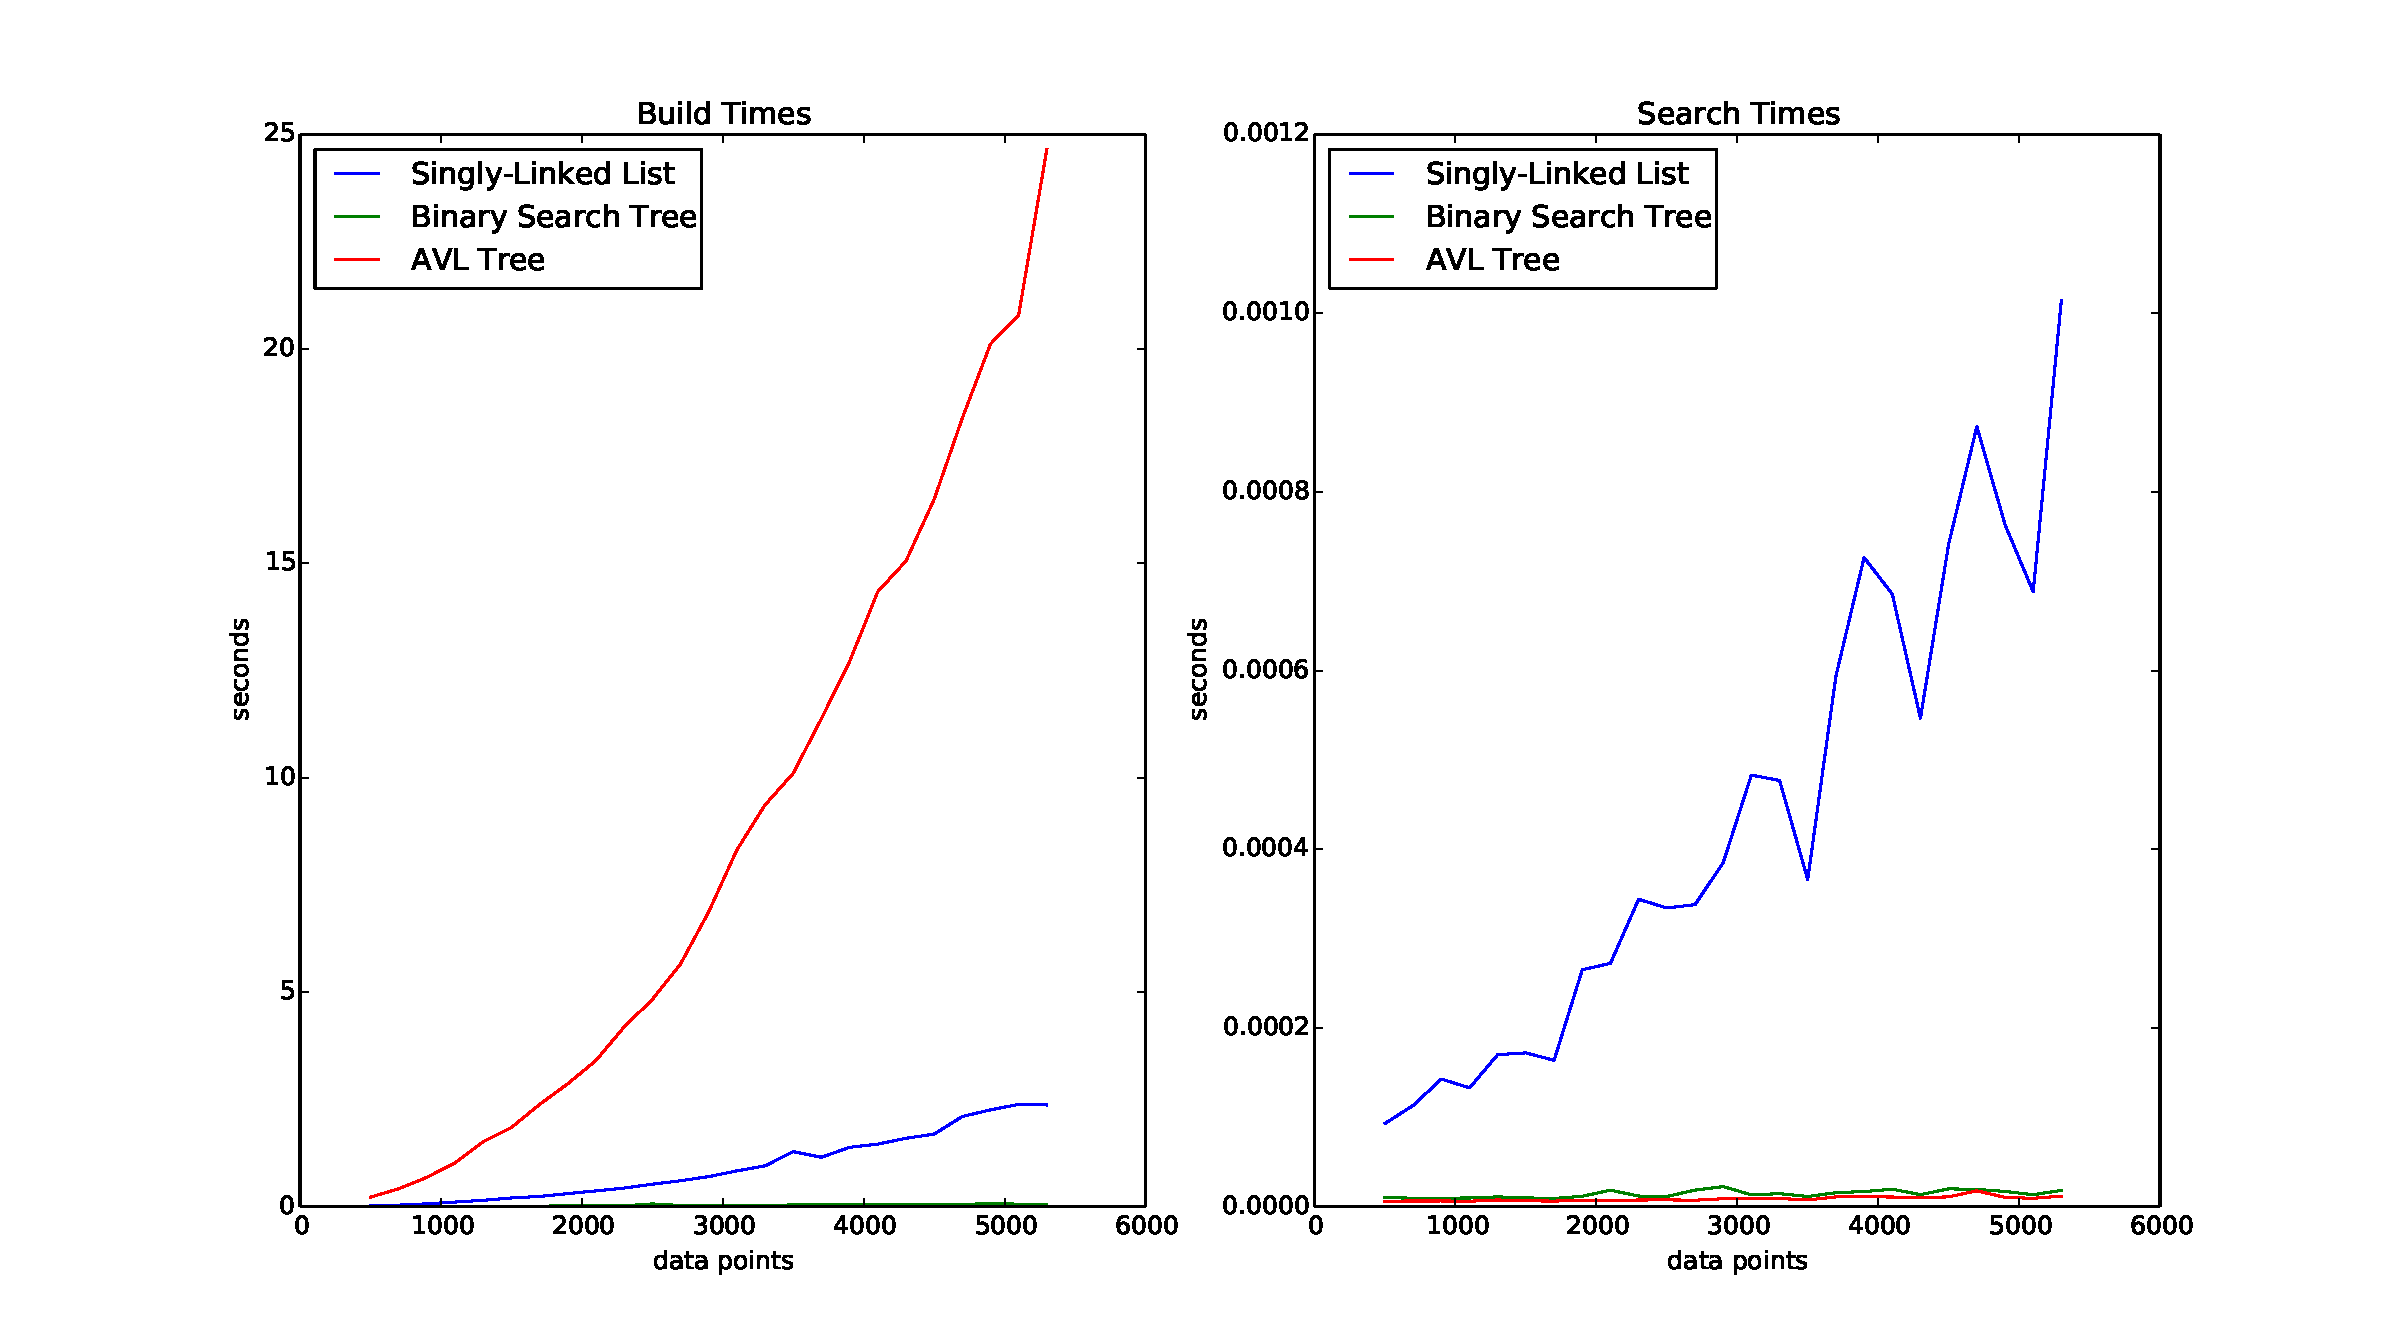
\includegraphics[width=\textwidth]{times.pdf}
\caption{Note that the \li{BST} has the fastest build times, but the \li{AVL} has the fastest search times. How would the graph change if the data were sorted to begin with?}
\label{fig:times}
\end{figure}

\end{problem}

